%%%%%%%%%%%%%%%%%%%%%%%%%%%%%%%%%%%%%%%%%%%%%%%%%%%%%%%%%%%%%%%





%%%%% CHOOSE PAGE LAYOUT
% The most common choices should be below.  You can also do other things, like replacing "a4paper" with "letterpaper", etc.

% This one will format for two-sided binding (ie left and right pages have mirror margins; blank pages inserted where needed):
\documentclass[a4paper,twoside]{lahcenthesis}
% This one will format for one-sided binding (ie left margin > right margin; no extra blank pages):
%\documentclass[a4paper]{lahcenthesis}
% This one will format for PDF output (ie equal margins, no extra blank pages):
%\documentclass[a4paper,nobind]{lahcenthesis} 



%%%%% SELECT YOUR DRAFT OPTIONS
% Three options going on here; use in any combination.  But remember to turn the first two off before
% generating a PDF to send to the printer!

% This adds a "DRAFT" footer to every normal page.  (The first page of each chapter is not a "normal" page.)
\fancyfoot[C]{\emph{DRAFT Printed on \today}}  

% This highlights (in blue) corrections marked with (for words) \mccorrect{blah} or (for whole
% paragraphs) \begin{mccorrection} . . . \end{mccorrection}.  This can be useful for sending a PDF of
% your corrected thesis to your examiners for review.  Turn it off, and the blue disappears.
\correctionstrue


%%%%% BIBLIOGRAPHY SETUP
% Note that your bibliography will require some tweaking depending on your department, preferred format, etc.
% The options included below are just very basic "sciencey" and "humanitiesey" options to get started.
% If you've not used LaTeX before, I recommend reading a little about biblatex/biber and getting started with it.
% If you're already a LaTeX pro and are used to natbib or something, modify as necessary.
% Either way, you'll have to choose and configure an appropriate bibliography format...

% The science-type option: numerical in-text citation with references in order of appearance.
\usepackage[style=numeric-comp, sorting=none, backend=biber, doi=false, isbn=false]{biblatex}
\newcommand*{\bibtitle}{References}

% The humanities-type option: author-year in-text citation with an alphabetical works cited.
%\usepackage[style=authoryear, sorting=nyt, backend=biber, maxcitenames=2, useprefix, doi=false, isbn=false]{biblatex}
%\newcommand*{\bibtitle}{Works Cited}

% This makes the bibliography left-aligned (not 'justified') and slightly smaller font.
\renewcommand*{\bibfont}{\raggedright\small}

% Change this to the name of your .bib file (usually exported from a citation manager like Zotero or EndNote).
\addbibresource{references.bib}


% Uncomment this if you want equation numbers per section (2.3.12), instead of per chapter (2.18):
%\numberwithin{equation}{subsection}



%%%%% THESIS / TITLE PAGE INFORMATION
% Everybody needs to complete the following:
\title{Fraud Detection}
\author{ your name }
\college{Goldsmiths College}

% Master's candidates who require the alternate title page (with candidate number and word count)
% must also un-comment and complete the following three lines:
%\masterssubmissiontrue
%\candidateno{933516}
%\wordcount{28,815}

% Uncomment the following line if your degree also includes exams (eg most masters):
%\renewcommand{\submittedtext}{Submitted in partial completion of the}
% Your full degree name.  (But remember that DPhils aren't "in" anything.  They're just DPhils.)
\degree{B. Computer Science}
% Term and year of submission, or date if your board requires (eg most masters)
\degreedate{\today}


%%%%% YOUR OWN PERSONAL MACROS
% This is a good place to dump your own LaTeX macros as they come up.

% To make text superscripts shortcuts
	\renewcommand{\th}{\textsuperscript{th}} % ex: I won 4\th place
	\newcommand{\nd}{\textsuperscript{nd}}
	\renewcommand{\st}{\textsuperscript{st}}
	\newcommand{\rd}{\textsuperscript{rd}}



%%%%% THE ACTUAL DOCUMENT STARTS HERE
\begin{document}



%%%%% CHOOSE YOUR LINE SPACING HERE
% This is the official option.  Use it for your submission copy and library copy:
\setlength{\textbaselineskip}{22pt plus2pt}
% This is closer spacing (about 1.5-spaced) that you might prefer for your personal copies:
%\setlength{\textbaselineskip}{18pt plus2pt minus1pt}

% You can set the spacing here for the roman-numbered pages (acknowledgements, table of contents, etc.)
\setlength{\frontmatterbaselineskip}{17pt plus1pt minus1pt}

% Leave this line alone; it gets things started for the real document.
\setlength{\baselineskip}{\textbaselineskip}


%%%%% CHOOSE YOUR SECTION NUMBERING DEPTH HERE
% You have two choices.  First, how far down are sections numbered?  (Below that, they're named but
% don't get numbers.)  Second, what level of section appears in the table of contents?  These don't have
% to match: you can have numbered sections that don't show up in the ToC, or unnumbered sections that
% do.  Throughout, 0 = chapter; 1 = section; 2 = subsection; 3 = subsubsection, 4 = paragraph...

% The level that gets a number:
\setcounter{secnumdepth}{2}
% The level that shows up in the ToC:
\setcounter{tocdepth}{2}


%%%%% ABSTRACT SEPARATE
% This is used to create the separate, one-page abstract that you are required to hand into the Exam
% Schools.  You can comment it out to generate a PDF for printing or whatnot.
\begin{abstractseparate}
	Your abstract text goes here.  
 % Create an abstract.tex file in the 'text' folder for your abstract.
\end{abstractseparate}


% JEM: Pages are roman numbered from here, though page numbers are invisible until ToC.  This is in
% keeping with most typesetting conventions.
\begin{romanpages}

% Title page is created here
\maketitle

%%%%% DEDICATION -- If you'd like one, un-comment the following.
%\begin{dedication}
%This thesis is dedicated to\\
%someone\\
%for some special reason\\
%\end{dedication}

%%%%% ACKNOWLEDGEMENTS -- Nothing to do here except comment out if you don't want it.
\begin{acknowledgements}
 	\subsection*{Personal}

This is where you thank your advisor, colleagues, and family and friends.


\subsection*{Institutional}

If you want to separate out your thanks for your college or dept.
\end{acknowledgements}

%%%%% ABSTRACT -- Nothing to do here except comment out if you don't want it.
\begin{abstract}
	Your abstract text goes here.  

\end{abstract}

%%%%% MINI TABLES
% This lays the groundwork for per-chapter, mini tables of contents.  Comment the following line
% (and remove \minitoc from the chapter files) if you don't want this.  Un-comment either of the
% next two lines if you want a per-chapter list of figures or tables.
\dominitoc % include a mini table of contents
%\dominilof  % include a mini list of figures
%\dominilot  % include a mini list of tables

% This aligns the bottom of the text of each page.  It generally makes things look better.
\flushbottom

% This is where the whole-document ToC appears:
\tableofcontents

\listoffigures
	\mtcaddchapter
% \mtcaddchapter is needed when adding a non-chapter (but chapter-like) entity to avoid confusing minitoc

% Uncomment to generate a list of tables:
%\listoftables
%	\mtcaddchapter

%%%%% LIST OF ABBREVIATIONS
% This example includes a list of abbreviations.  Look at text/abbreviations.tex to see how that file is
% formatted.  The template can handle any kind of list though, so this might be a good place for a
% glossary, etc.
% First parameter can be changed eg to "Glossary" or something.
% Second parameter is the max length of bold terms.
\begin{mclistof}{List of Abbreviations}{3.2cm}

\item[NLG] Natural Language Generation - the field of research dedicated to the computational generation of natural sounding text.

\item[NLP] Natural Language Processing - the field of research dedicated to the understanding and processing of human language.



\end{mclistof} 


% The Roman pages, like the Roman Empire, must come to its inevitable close.
\end{romanpages}


%%%%% CHAPTERS
% Add or remove any chapters you'd like here, by file name (excluding '.tex'):
\flushbottom

%\begin{savequote}[8cm]
%\textlatin{Neque porro quisquam est qui dolorem ipsum quia dolor sit amet, consectetur, adipisci velit...}
%
%There is no one who loves pain itself, who seeks after it and wants to have it, simply because it is pain...
%  \qauthor{--- Cicero's \textit{de Finibus Bonorum et Malorum}}
%\end{savequote}

\chapter{\label{ch:1-intro}Introduction} 

\minitoc

\section{Overview of the System}
This project attempts to create believable reviews for a movie given a corpus of text (such as reviews of that specific film taken from users of IMdB) which discusses it. 

There are a collection of systems I have implemented for this project which range from simple to greater complexity, which attempt to create believable text in review or discursive form. \\

The first system is a review website created in PHP, using a MySQL database to host content, which host movie reviews generated as well as to be a platform for collecting user data, feedback and analytics. As well as this system - a further PHP website for comparative review testing has been created to supplement the gathering of feedback.\\

The second system is a bot for the website Twitter, which uses Markov chains to reply to tweets discussing movies and post discussion in the tags for specific films, in order to drive traffic towards the review website as well as explore the ability of Markov chains to generate believable text.\\

The next system is a collection of methods used in generating reviews for movies. The first being the use of a Markov Chain model on a corpus of movie review text. Next, which aims to be more insightful is a template-based system which mines sentiment from a corpus of text about a specific film as part of speech tagging to create text based on opinions expressed in the corpus of text given, and outputs a structured review. The third system attempts to use a Natural Language Generation methodology in creating a review, following the 5 part methodology proposed by Dale and Reiter.

\section{Motivation}

The Internet is a vast resource for opinion, thoughts and discourse on many topics such as film and other media. There are countless reviews, ratings and comments about any given topic, and this is a valuable resource to mine in order to extract opinion and detail about what is being discussed.\\

The applications of Natural Language Processing (NLP) and more specifically Natural Language Generation (NLG) are powerful in this domain.  Opinion mining and understanding of such a vast field of reviewers and people engaging in discussion can provide interesting data and context on the success of a film. Such methods are able to process and understand a very large corpus of text far faster than one may be able to read through all of the writings on a film manually. \\

This project aims to create a system that addresses these issues, and generates a review of a movie that is both coherent and insightful, related to the corpus of movie review text it is given. It would prefer to be somewhat summarative of the corpus it is given, but due to the natural polarity of movie review text it would be difficult to engineer and assess quite how summarative a piece of work may be.\\

A system of this kind could be employed in business - for example, reviews and articles about cinema can have a profound effect on their commercial success, and if enough respected reviewers pan a film it may become necessary to understand why - and a tool such as this could aid this process.\\

It could also be employed at a consumer level in order for a user to quickly evaluate whether or not they wanted to watch a film or buy a product based on a vast amount of review text that exists rather than the opinion of a singular reviewer.\\
As well as this, it may simply be used for entertainment purposes, to fool or generate conversation about a film in particular.\\

\section{Thesis Structure}
This thesis is structured as follows:\\
Chapter 2: This chapter provides background research into generating prose as well as evaluating text and a review of literature in these topics.\\ It also includes an exploration of past works in similar generative projects as well as human-like text agents such as Twitter bots.\\
Chapter 3: A specification of the project, including the design and implementation details of the systems discussed in this dissertation.\\
Chapter 5: Testing of the systems performed are documented in this chapter.\\
Chapter 6: An evaluation of the systems created.\\
Chapter 7: A conclusion, discussing the outcomes of the systems implemented.\\
After this, a bibliography and appendices section are included.


%\begin{savequote}[8cm]
%Alles Gescheite ist schon gedacht worden.\\
%Man muss nur versuchen, es noch einmal zu denken.
%
%All intelligent thoughts have already been thought;\\
%what is necessary is only to try to think them again.
%  \qauthor{--- Johann Wolfgang von Goethe \cite{von_goethe_wilhelm_1829}}
%\end{savequote}

\chapter{\label{ch:2-litreview}Background}

%\minitoc

\section{Introduction}

This document introduction won't serve as a complete primer on \LaTeX.  There are plenty of those online, and googling your questions will often get you answers, especially from \url{http://tex.stackexchange.com}.

Instead, let's talk a little about a few of the features and packages lumped into this template situation.  The \verb|savequote| environment at the beginning of chapters can add some wittiness to your thesis.  If you don't like the quotes, just remove that block.

For when it comes time to do corrections, there are two useful commands here.  First, the \verb|mccorrect| command allows you to highlight a short correction \mccorrect{like this one}.  When the thesis is typeset normally, the correction will just appear as part of the text.  However, when you declare \verb|\correctionstrue| in the main \verb|Oxford_Thesis.tex| file, that correction will be highlighted in blue.  That might be useful for submitting a post-viva, corrected copy to your examiners so they can quickly verify you've completed the task.

\begin{mccorrection}
For larger chunks, like this paragraph or indeed entire figures, you can use the \verb|mccorrection| environment.  This environment highlights paragraph-sized and larger blocks with the same blue colour.
\end{mccorrection}

Read through the \verb|final-report.tex| file to see the various options for one- and two-sided printing, including or excluding the separate abstract page, and turning corrections and draft footer on or off, and the separate option to centre your text on the page (for PDF submission) or offset it (for binding).  There is also a separate option for master's degree submissions, which changes identifying information to candidate number and includes a word count.  (Unfortunately, \LaTeX has a hard time doing word counts automatically, so you'll have to enter the count manually if you require this.)

\section{Fraud Detection}
\label{app:fraud}

Within months of Röntgen's discovery of the X-ray in \mccorrect{1895}\cite{gagliardi_rontgen_1996}, cardiac pathology was being investigated via non-invasive imaging \cite{gagliardi_cardiac_1996}.  Over the intervening years, cardiac imaging modalities and techniques have advanced significantly.  Clinically, cardiac imaging is used for two broad purposes: diagnosis of pathophysiology and guidance of interventional procedures.  These applications impose different requirements on imaging equipment, image acquisition time, computational complexity, spatial and temporal resolution, and tissue discrimination.  The common diagnostic and interventional cardiac imaging techniques in current clinical practice are reviewed below.  An accessible introduction to the physics of medical imaging can be found in Webb's \textit{Introduction to Biomedical Imaging} \cite{webb_introduction_2002}.  A comprehensive overview of the use of imaging in clinical cardiology is presented in Leeson's \textit{Cardiovascular Imaging} \cite{leeson_cardiovascular_2011}.

\subsection{Machine Learning}
\label{sub:machine-learning}

Beyond the chest X-ray (`plain film'), the key non-invasive imaging modalities in diagnostic cardiology are echocardiography, magnetic resonance imaging, and X-ray computed tomography, which are reviewed below.  Nuclear medicine, including positron emission tomography (PET) and single-photon emission computed tomography (SPECT), are not discussed here, as they do not play a role in the chapters to follow.

\subsubsection{Recurrent Neural Network}
Most all previous RNN based~\emph{dst~forecasting}
research~\cite{pallocchia:2006} has relied on
batch\footnote{batch refers to models trained on an in sample data
set and then evaluated on an out of sample data set in which no
learning occurs in the out of sample data set.} algorithms for
training the RNN. Batch training algorithms are unable to
incorporate newly arrived information into the model parameters
without re-processing the entire data set (which is a costly
operation). Furthermore, the training algorithms used thus far for
training the RNNs on~\emph{dst~forecasting} (all of which have been batch
first order gradient descent) are known to be susceptible to local
minima, and uncertain convergence. This has been a bottleneck in the
area (and may stifle future progress in neural based forecasting of
geomagnetic phenomena), as well performing models are difficult to
obtain, and new events can not readily be incorporated into the
model for improved forecasts.


\begin{figure}
\centering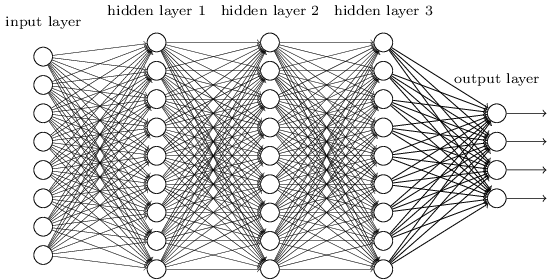
\includegraphics[width=0.7\textwidth]{figures/rnn.png} 
\caption[A schematic representation of the fully recurrent neural
network architecture.]{A schematic representation of the fully recurrent neural
network architecture}
\label{fig:fourchamber}\end{figure}


\subsubsection{Rand Index Algorithm}

%\begin{figure}
%\centering\includegraphics[width=0.7\textwidth]{figures/sample/Gray498.png} 
%\caption[Four-chamber illustration of the human heart.]{Four-chamber illustration of the human heart.  Clockwise from upper-left: right atrium, left atrium, left ventricle, right ventricle.}
%\label{fig:fourchamber}\end{figure}







The use of acoustic waves for medical diagnosis, inspired by naval sonar, was initially developed in the 1940s \cite{gagliardi_ultrasonography_1996}.  By 1954, the first clinically useful cardiac ultrasound -- examining motion of the mitral valve in stenosis -- was reported \cite{edler_ultrasonic_1957}.  These early scans were one-dimensional images (`A-mode'), sometimes repeated to generate a time axis (`M-mode').   The sector-scanning probe was developed in the 1970s \cite{bom_ultrasonic_1971,griffith_sector_1974}, leading to the `B-mode' that a modern cardiologist would recognise as an echocardiogram.



\chapter{\label{ch:3-design} Design}

%\minitoc

\section{Introduction}

\section{Aims and Objectives}
\subsection{Aims}

The primary aim of this project is to explore methods for text generation and then develop a system through which prose about movies can be generated. This prose should be in the form of a movie review, and should pick the most recurrent points or themes in a corpus of movie reviews discussing a singular movie.

\subsection{Objectives}

To develop a natural language generation system which picks points from multiple review texts and uses them to structure an informed review.\\
To develop an online platform to host generated movie reviews which can gather feedback and data on the reception of said review.\\
To develop an autonomous bot that can discuss movies (or at least reply with an opinion of a movie) over twitter. Ideally this would drive traffic towards the movie review blog which hosts reviews made by the bot.

\section{Movie Review Generation}

\subsection{Markov Chain for Text Generation}
\subsection{Template-Based System for Text Generation}
The design of this system started with the premise of filling out template sentences for segments of a review in a random fashion until a text of a satisfactory size is produced. The initial idea being that an introduction is filled in, then a brief plot synopsis, some text evaluating the performances of actors and noteworthy crew (such as the director or writers) and then a closing statement regarding whether or not its worth seeing a film.\\

The first step of the template system is data gathering.

It web scrapes a corpus of movie reviews for a given movie from IMdB. These are user reviews taken from a movie's reviews page, and an amount are taken sorted by their highest rating. Then it web scrapes plot synopsis, also from IMdB this is then summarized using the TextRank algorithm. It finally uses themoviedb's API to gather metadata about a film, such as cast crew and genre.\\


The second step in this process is then forming an understanding of that data.
First is the separation each review text into a large list of sentences so that they can be tagged and analyzed for sentiment.
Categorise each sentence as about a particular topic or person (cast, crew, director), using the metadata gathered from the OMdB API to match sentences to these topics.\\

The final step is then filling in the reviews templates until completion.
Builds an introduction based on a template, a plot summary after that, a body of review text, and then a closing statement based on the template.
Templates are filled with words determined by sentiment, and adjectives and adverbs mined from part of speech tagging sentences regarding the topic discussed in the template sentence.\\


\subsection{NLG System}

\section{Twitter Bot}
The Twitter bot exists in order to drive traffic towards the reviews generated and also act as a test of generating text in shorter formats than review - for example the markov chains discussed earlier are much more believable if you don't let them go on for too long. The limit of 144 characters is certainly suitable for this.\\
The bot itself uses a twitter API wrapper called Tweepy, which handles Twitter API requests required in order to make posts, search and navigate twitter.\\
There are a number of behaviours programmed for the bot to gather attention and direct users towards the website. The first is simply the automated posting of links to movie reviews generated, with a template message that reads along the lines of "Read my review for #filmname here".\\
The next behaviour is replying to posts which have been identified to be about the movie in question with comments generated from a markov chain of other tweets about the movie.\\ 


\section{Blog Website}
The design of the blog website is relatively simple. It is a Wordpress-like blogging website written in PHP, wish a MySQL database that stores the reviews, user information and the comments made and analytics for the site.\\
I have chosen MySQL and PHP as they are languages I am familiar with, and have worked using before, as well as their being suitable for the task of a small blogging platform.\\
The website itself is a front-page which lists paginated results for movie reviews written by the movie review generator, an interface for making/creating posts, and a way to view the reviews in full. It also has user comments for gathering qualitative feedback and page visits and engagements are tracked using Google analytics and a MySQL hit-counter.\\



\chapter{\label{ch:4-implementation} Implementation}

%\minitoc

\section{Introduction}

\section{Movie Review Generation}

\section{Blog Website}

\section{Twitter Bot}



\chapter{\label{ch:5-testing} Testing}

%\minitoc

\section{Introduction}
Testing each part of this system involves checking primarily that outputs are what they should be, but also checking that the data scraped from the internet is handled correctly in edge-cases and that errors are handled correctly and not ignored or allowed to halt the program code. Because of this, I have to create my own example data that looks like what is gathered from web scraping and API calls which mirror edge-cases.

\section{Movie Review Generation}
\subsection{Testing of Review Generation}
This involved a lot of testing of individual modules and functions to make sure that they handle all the data passed in to them. As the completed system merely takes an input which is the name of a film and several on/off parameters, there is not much in the user space that can change with regards to testing.
\subsection{Changes Made}
\section{Blog Website}
\subsection{Testing of Blog Website}
Most of this testing work is making sure that the SQL CRUD functions work, and making sure that the website displays the information that is intended, and checking that my information gathering here is accurate.
\subsection{Changes Made}
\section{Twitter Bot}
\subsection{Testing of Twitter Bot}
I have decided to test the Twitter Bot with a series of items which I have saved to use for testing, as well as some live tests taken from Twitter at runtime. 
\subsection{Changes Made}


\chapter{\label{ch:7-conclusion} Conclusion and Future Work}

%\minitoc


\section{Review of Aims and Objectives}
I would say that this project has been moderately successful. Some feasible movie review text has indeed been generated, although not a lot and not in quite as large quantity or variety as I had aimed.
\subsection{Aims}
The aim of this project was to generate movie review prose that passed as human. This has been partially achieved, at the sentence level, although a movie review generated by any of my systems is not likely to pass as human, mostly due to the falling-apart of coherence outside of reporting facts and sentiments. I would not say this was achieved with great success, as little interaction with any of the systems aiming to pass as human has occurred.
\subsection{Objectives}
To explore methods for generating text which reviews film.\\
This object has certainly been met. I have explored a number of options for generating prose and implemented several methods for generating prose. I have looked at Markov models, Feed-Forward Neural Networks, Template based systems using context-free grammars, and Natural Language Generation architectures for generating prose.\\

To develop a natural language generation system which picks points from multiple review texts and uses them to structure an informed review.\\
Although I have implemented a system to meet his goal, the outputs generated do not manage to pass as human, and therefore I would not say I have met this objective with great success. As well as this, I made the concession of including templates into the NLG system in an attempt at making the system more human-like. More time to work on this system and I feel I could have met this objective more, although it would be partially template-based rather than strictly NLG.\\
To develop an online platform to host generated movie reviews which can gather feedback and data on the reception of said review.\\
I have met this objective successfully, although it had not been used as much as I had hoped for the collection of data. I could have put more time into the development of the site in order to make it more welcoming as well as hosting it on a URL that is potentially less scary than the URL of my system. (doc.gold.ac.uk/~tpalm003/reviews/index.php).\\
To develop an autonomous bot that can discuss movies (or at least reply with an opinion of a movie) over twitter. Ideally this would drive traffic towards the movie review blog which hosts reviews made by the bot.\\
This goal has been met, although its outreach is limited by the behaviours it puts into place. It makes posts and can post with hash-tags in an attempt to reach an audience, but it does not engage with twitter users through other interactions which would arguably make it a more believable bot, and at the very least have it seen by more people.\\


\section{Lessons Learned}
I have learned a number of things from this project, and had I started it again have a number of things I would do differently.
At the programming level, I've learnt a lot about using APIs as well as interracting with XML and JSON objects, as well as parsing text and working around very error-prone systems such as requesting data that might not necessarily exist.\\
I have had to research language processing and sentiment tagging, although I did opt to use libraries for these in my implementation as there was little point reimplementing code for systems with so many interacting elements.\\
I'd also not recommend relying on user data for systems that require finding attention in the real world (rather than appealing to users for feedback), as this has proven to be difficult to manage. As well as this I would recommend that people choose less subjective topics to implement NLG systems for if they were to choose NLG as a dissertation topic.


\section{Future Work}


\subsection{Improvements to current work}
An interesting area to explore is expanding the Twitter bot to handle behaviours other than self promotion and Markov chain generated text to reply to others. This would enable a system which intended to draw more attention to itself to operate in a more human-like manner as a real twitter user is more likely to utilize all of the features of the website and have a greater outreach through the use of replies - as notifications are sent directly to the user rather than having to search for a tweet generated by the bot.\\


It would also be interesting to expand the NLG system to handle a larger range of topics within movie generation for a more believable and comprehensive review of the film, and expand the grammars used to generate the sentiment-driven sentences. This would mostly include much more specific sentiment analysis using lists of sentiment tagged words for specific topics and themes that occur in cinema.\\

A further interesting expansion would be to target reviews at different audiences where people actively read for them, such as Youtube comments, reviews for Amazon streaming videos, and other websites that host users movie watchlists and reivews such as IMdB and letterboxd, as they have active communities that use will read these reviews to gage whether or not they want to watch a film, or for other purposes such as validating their own opinions. 

\section{The Future of Generative Film Reviews}
It is definitely safe to assume that the human-written review will not be made obsolete by reviews created from NLG methods for a long while yet. Given that a system like this would need to build its knowledge from some agent with enough insight to identify talking points and provide sentiment for each of these talking points, it is safe to say that without brilliant leaps in computer vision and audio processing, an article penned by a trusted reviewer is not going to be made redundant any time soon.









%% APPENDICES %% 
% Starts lettered appendices, adds a heading in table of contents, and adds a
%    page that just says "Appendices" to signal the end of your main text.
\startappendices
% Add or remove any appendices you'd like here:




\chapter{Evaluation Data}
\subsection{Twitter Analytics Data}



\centering
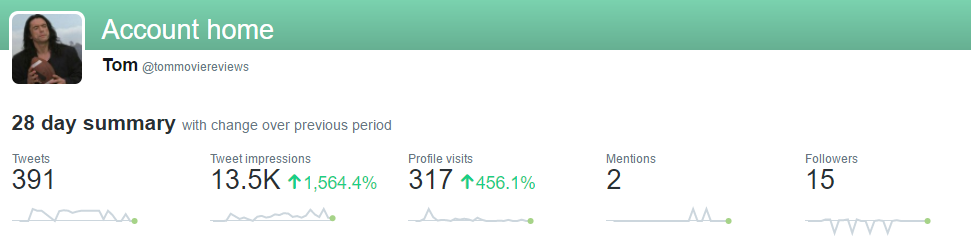
\includegraphics[width=0.7\linewidth]{figures/twitter_analytics/28daysummary}
%\caption{28 Day Summary of Twitter Bot Analytics}
\label{fig:28daysummary}


\centering
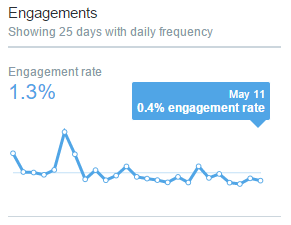
\includegraphics[width=0.7\linewidth]{figures/twitter_analytics/engagements}
%\caption{Total number of 'engagements' with twitter bot over active period}
\label{fig:engagements}


\centering
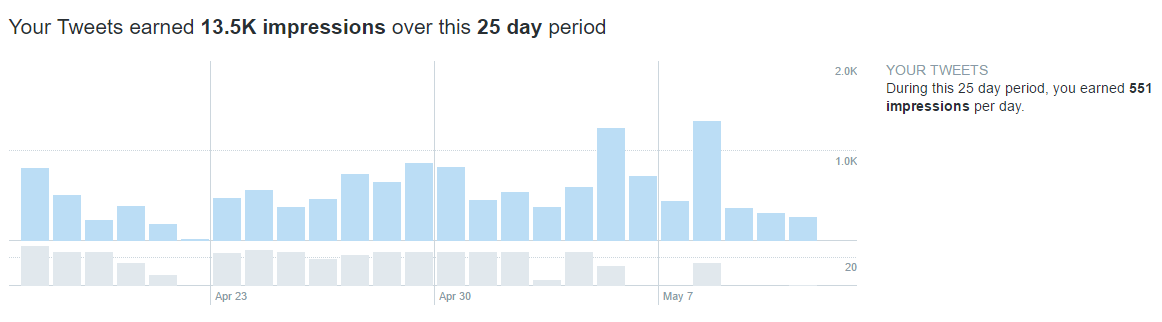
\includegraphics[width=0.7\linewidth]{figures/twitter_analytics/impressions}
%\caption{Total number of 'impressions' made by twitter bot over active period}
\label{fig:impressions}


\centering
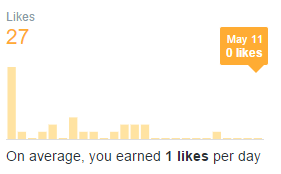
\includegraphics[width=0.7\linewidth]{figures/twitter_analytics/likes}
%\caption{Likes obtained over active period}
\label{fig:likes}

\centering
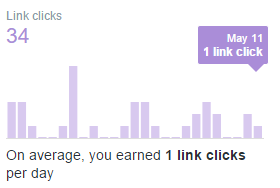
\includegraphics[width=0.7\linewidth]{figures/twitter_analytics/linkclicks}
%\caption{Links clicked over active period}
\label{fig:linkclicks}

\centering
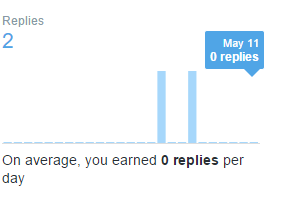
\includegraphics[width=0.7\linewidth]{figures/twitter_analytics/replies}
%\caption{Replies to posts made by bot over active period}
\label{fig:replies}

\centering
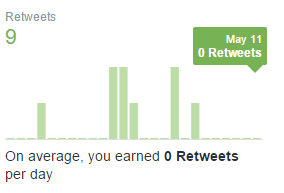
\includegraphics[width=0.7\linewidth]{figures/twitter_analytics/retweets}
%\caption{Retweets of posts made by bot over active period}
\label{fig:retweets}




\subsection{Google Analytics Data}

\centering
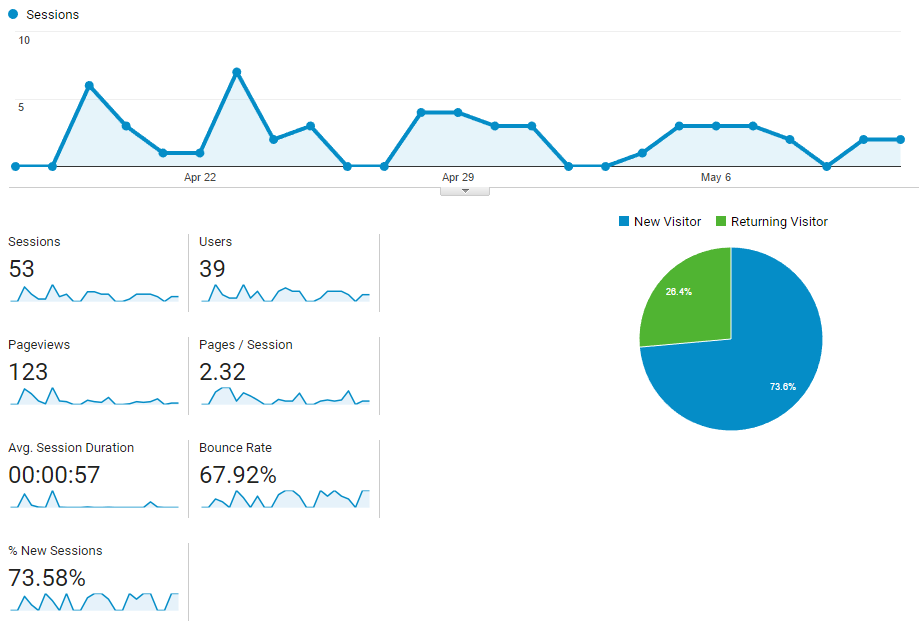
\includegraphics[width=0.7\linewidth]{figures/google_analytics/uniqueSessions}
%\caption{Google Analytics Screenshot showing unique sessions over test period}
\label{fig:uniquesessions}

\centering
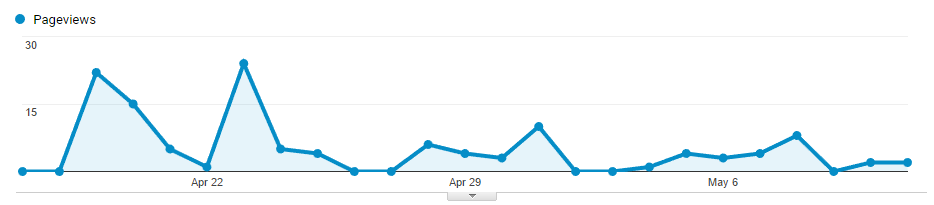
\includegraphics[width=0.7\linewidth]{figures/google_analytics/pageviews}
%\caption{Google Analytics Screenshot showing pageviews over test period}
\label{fig:pageviews}

\centering
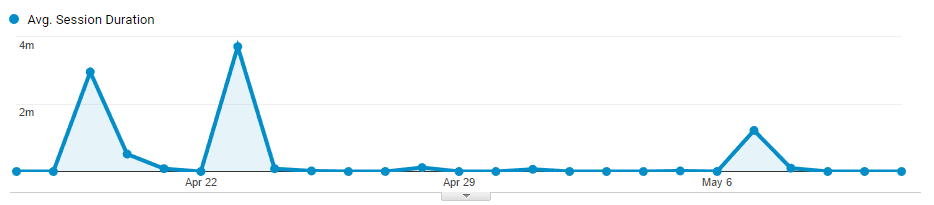
\includegraphics[width=0.7\linewidth]{figures/google_analytics/sessionDuration}
%\caption{Google Analytics Screenshot showing average session duration over test period}
\label{fig:sessionduration}

\chapter{Turing-Like Test Results}


\includepdf[pages={1-},scale=1]{"figures/turinglike_results/Review Feedback - reviewExcerpt (1)"}      


\chapter{Preliminary Project Report}


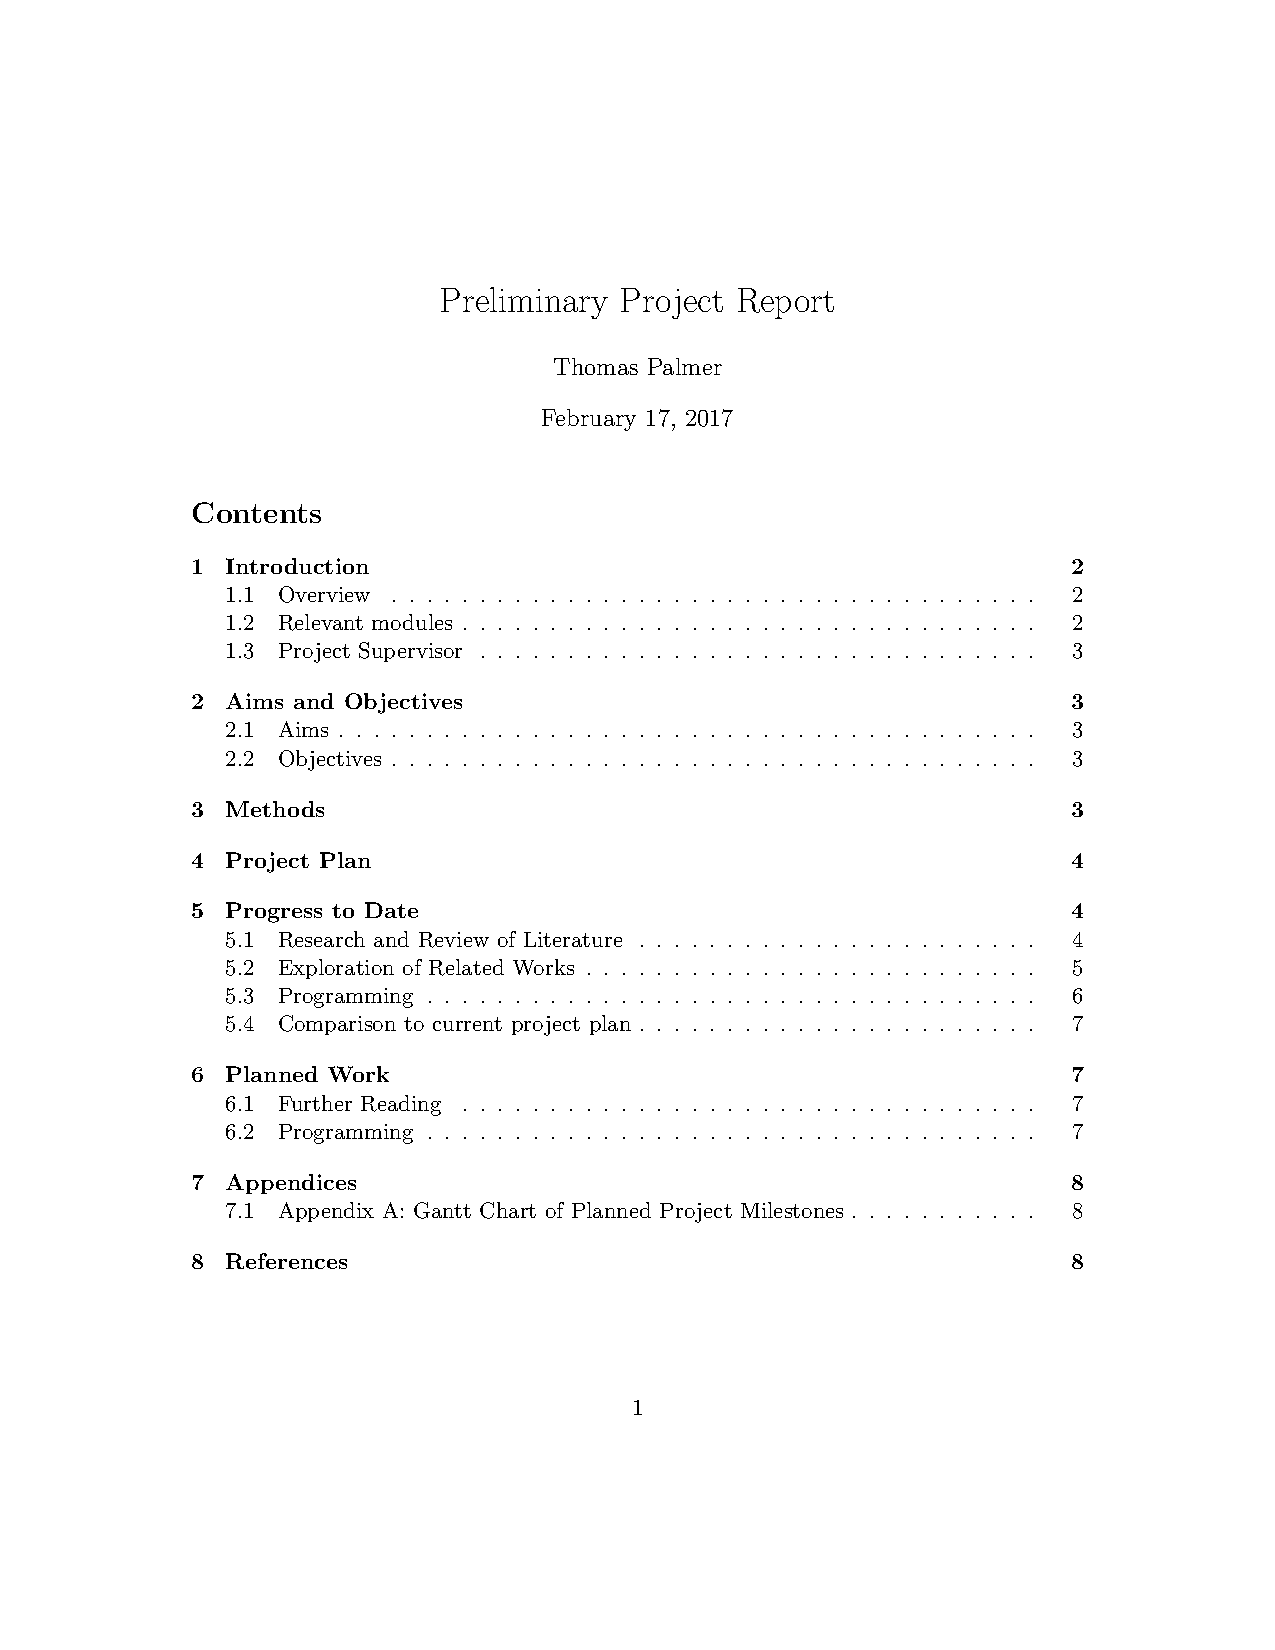
\includepdf[pages={1-},scale=1]{figures/preliminaryReport2}



\chapter{Project Logs}
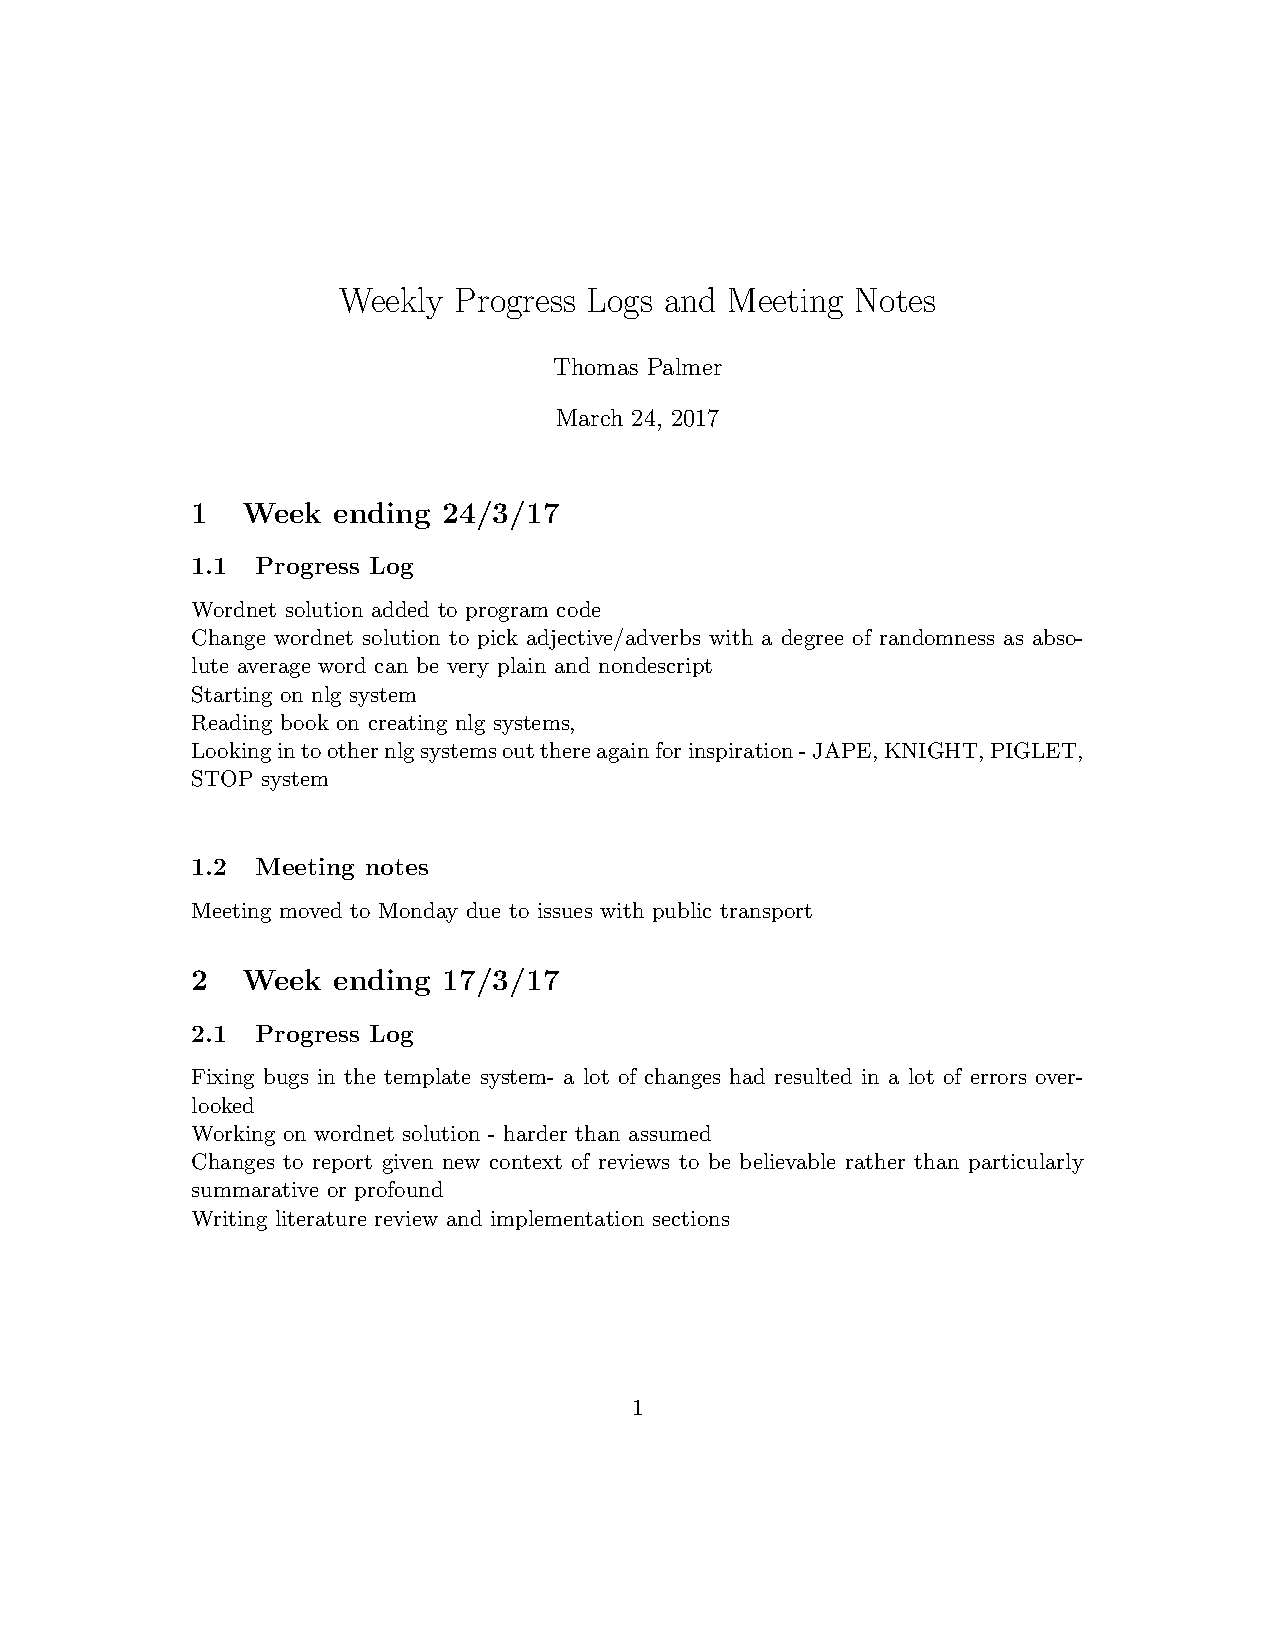
\includepdf[pages={1-}, scale=1]{figures/meetingnotes_17-03-24_thomas-palmer}

\chapter{Program Code}

\subsection{Python}
\subsection{PHP}
\subsection{mySQL}


%%%%% REFERENCES


\setlength{\baselineskip}{0pt} % JEM: Single-space References

{\renewcommand*\MakeUppercase[1]{#1}%
\printbibliography[heading=bibintoc,title={\bibtitle}]}



\end{document}
